\section{Anwendung}
\label{sec:anwendung}
\subsection{Seitenstruktur}

Alle Seiten der Anwendung sind nach dem gleichen Muster aufgebaut. Sie werden von der Datei \code{index.php} erzeugt. Hier werden wie in Abbildung \ref{fig:struktur} auf Seite \pageref{fig:struktur} die Seitenelemente aus den verschiedenen Include--Dateien für den Kopfbereich, die Navigationsleiste am rechten Rand und dem Fußbereich zusammengesetzt\footnote{Darstellung vereinfacht}. Der eigentliche Funktionsbereich\footnote{Frage anzeigen, Antworten speichern und auswerten, anmelden, abmelden, Eingabemaske für neue Fragen sowie das Abspeichern der neuen Fragen} werden von den PHP--Dateien im Verzeichniss \code{.../pages/} übernommen.

\begin{figure}[h]
\begin{spacing}{1.0}	
\begin{minted}[bgcolor=bg]{php}
<?php 
  include($_SERVER['DOCUMENT_ROOT'].'/includes/header.php'); 
?>
<div class="row">
 <div class="col-md-8">
  <?php 
    include($_SERVER['DOCUMENT_ROOT'].'/pages/'. $show . '.php'); 
  ?> 
 </div>
 <div class="col-md-4">
  <?php 
    include($_SERVER['DOCUMENT_ROOT'].'/includes/sidebar.php'); 
  ?>
 </div>	  
</div>
<?php 
  include($_SERVER['DOCUMENT_ROOT'].'/includes/footer.php'); 
?>
\end{minted}
\caption{HTML: Seitenstruktur und PHP--Includes}
\label{fig:struktur}
\end{spacing}
\end{figure}

Diese Seitenelemente und Programmteile werden in einer Struktur aus \code{DIV}--Ele\-menten angeordnet, welche durch die CSS--Klassen des Bootstrap--Frameworks zu einem modernen, responsiven Layout ausgezeichnet werden. Der Anwendungsentwickler braucht sich somit nicht um die optimale Darstellung der HTML--Seiten auf Desktoprechnern, Tabletts oder Smartphones zu kümmern. Jede Bildschirmgröße erhält durch Bootstrap automatisch ein speziell abgestimmtes Layout.

\subsection{Layoutanpassungen mit CSS}

Die Gestaltung des Layouts mit „Cascading Stylesheets“ (kurz: CSS) ermöglicht es, das durch das Bootstrap--Framework vorgegebene Aussehen durch hinzufügen eines eigenen Stylesheets anzupassen.

So wurden bei der besprochenen Anwendung die Überschriften in der Seitenleiste individuell Farbig unterstrichen. Die Thematischen Blöcker werden hierzu in \code{DIV}--Blöcken mit den entsprechenden CSS--IDs eingeschlossen. Wie in Abbildung \ref{fig:seitenleiste} auf Seite \pageref{fig:seitenleiste} zu sehen, werden die Links beim berühren mit dem Mauszeiger in der gleichen Farbe dargestellt.

Bei der Darstellung der Auswertung werden die vom Benutzer selbst gegebenen Antworten durch Auszeichnung mit einer CSS-Klasse in fetter Schrift hervorgehoben. 

\begin{figure}[h]
\begin{center}
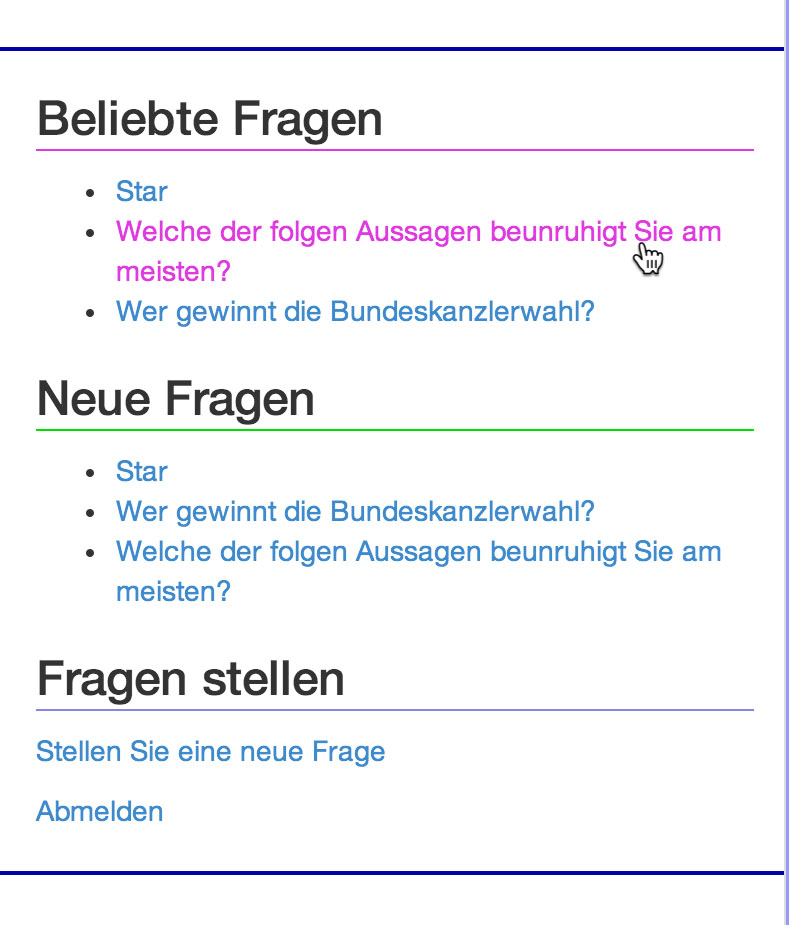
\includegraphics[width=\textwidth]{seitenleiste.jpg}
\caption{Unterstreichungen und Hervorhebungen per CSS}
\label{fig:seitenleiste}
\end{center}
\end{figure}

\subsection{Mögliche Benutzerpfade durch die Anwendung}

Abbildung \ref{fig:zustaende} auf Seite \pageref{fig:zustaende} zeigt die Pfade, auf denen der Nutzer durch die Anwendung navigieren kann. Hierbei wurde die Darstellung wegen der besseren Übersichtlichkeit auf den jeweiligen Erfolgsfall reduziert. Bei einem Anmeldefehler erscheint direkt wieder das Anmeldeformular. Bei Datenbankfehlern (z.B. beim Abspeichern einer neuen Frage) erscheint die entsprechende PHP--Fehlermeldung.

\begin{figure}[h]
\begin{center}
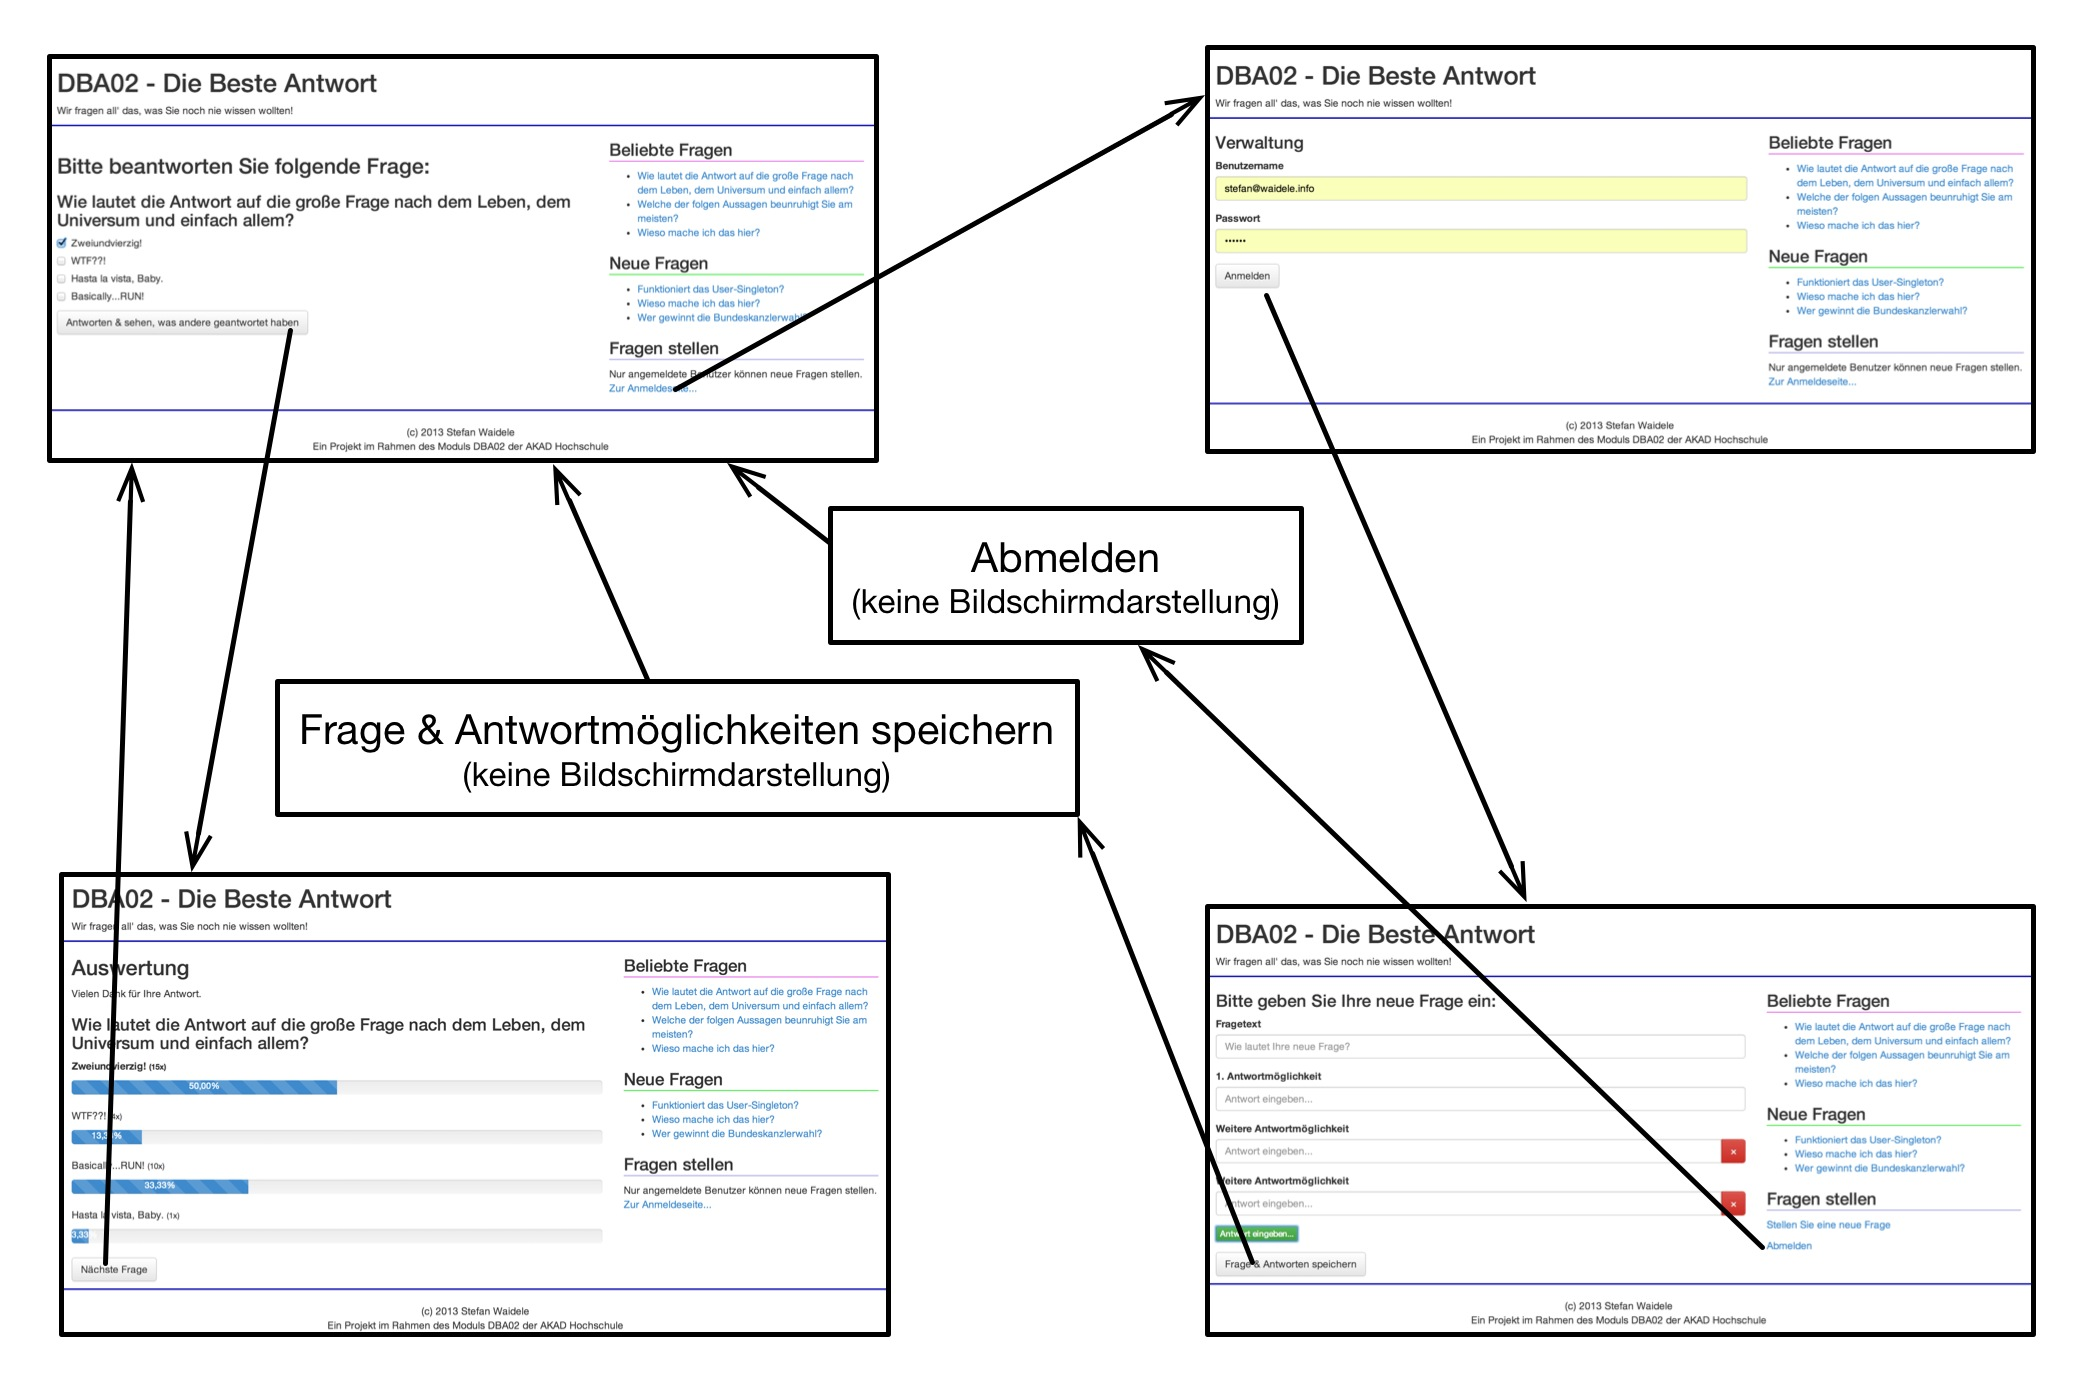
\includegraphics[width=\textwidth]{zustaende.jpg}
\caption{HTML--Seiten und Verlinkungen}
\label{fig:zustaende}
\end{center}
\end{figure}

\subsection{Eingabeformular für neue Fragen}

Zunächst stellt das Eingabeformular für neue Fragen und Antwortmöglichkeiten ein HTML--Formular dar, dessen Grundstruktur in Abbildung \ref{html:inputform} gezeigt wird. 

\begin{figure}[h]
\begin{spacing}{1.0}
\begin{minted}[bgcolor=bg]{html}
<form action="/index.php?show=speichern" method="post">
  <input type="text" name="frage" >
  <input type="text" name='awm[]' >
  <button type="button">
    Antwort eingeben...
  </button>
  <button type="submit">
    Frage &amp; Antworten speichern
  </button>
</form>
\end{minted}
\caption{HTML: Eingabeformular (vereinfacht)}
\label{html:inputform}
\end{spacing}
\end{figure}

Hierbei ist zu beachten, dass lediglich ein Feld zur Eingabe einer einzigen Antwort zur Verfügung steht. Der HTML--Button mit der Aufschrift „Antwort eingeben...“ wird daher mit einer JavaScript--Funktion belegt, die ein weiteres Antwortfeld an der entsprechenden Stelle\footnote{d.h. am Ende des Elements mit der ID „answers“} im DOM-Baum\footnote{DOM: Document Object Model, Browserinternes Interface zur Darstellung und Manipulation des HTML--Dokuments. Siehe auch \url{http://www.w3.org/DOM/}} einfügt. Hierzu werden die vom jQuery--Framework bereitgestellten Funktionen genutzt. Diese übernehmen auch das optisch ansprechende Einblenden des neuen Felds.

\begin{figure}[H]
\begin{spacing}{1.0}
\begin{minted}[bgcolor=bg]{javascript}
$("#newanswer").click(function() {
  var na = $("HTML-Code: Weiteres Eingabefeld mit Button");
  na.hide();
  na.appendTo("#answers");
  na.slideDown();	
});
\end{minted}
\caption{jQuery: Weiteres Eingabefeld (vereinfacht)}
\label{jquery:weitereantwort}
\end{spacing}
\end{figure}

Im Gegensatz zur ersten Antwortmöglichkeit sind alle weiteren Antwortmöglichkeiten mit einem HTML--Button versehen, der es erlaubt diese wieder zu löschen. Auch hierzu wird dem Button eine JavaScript--Funktion zugewiesen, die mithilfe von jQuery für das Ausblenden und Entfernen des Eingabefelds aus dem DOM--Baum sorgt:

\begin{figure}[H]
\begin{spacing}{1.0}
\begin{minted}[bgcolor=bg]{javascript}
$(".delanswer").click(function(){
 $(this).parent().parent().parent().slideUp("normal",
 function() {$(this).remove();}
);
\end{minted}
\caption{jQuery: Eingabefeld löschen (vereinfacht)}
\label{jquery:antwortloeschen}
\end{spacing}
\end{figure}

Durch Klicken des Buttons mit der Aufschrift „Frage \& Antworten speichern“ sendet der Nutzer die eingegebenen Werte an das PHP--Script unter \code{.../pages/speichern.php}. Da alle Antwort--Eingabefelder ein gleichlautendes \code{name}--Attribut besitzen, werden die Antwortmöglichkeiten dem Script in einem Array übergeben, welches der in Abschnitt \ref{sec:speichern} beschriebenen Methode der Klasse „SQL“ übergeben wird.

\subsection{Benutzerverwaltung}

Wie in Abschnitt \ref{sec:user} beschrieben stellt die Klasse „user“ alle Funktionen für die Authentifizierung der Seitenadministratoren bereit. Das PHP--Script unter \code{.../pages/anmeldung.php“} nimmt daher lediglich den Benutzernamen und das Passwort über ein HTML--Formular entgegen und übergibt diese der Methode \code{User::auth()}.

Alle Teile der Anwendung erhalten über den in Abbildung \ref{php:getinstance} gezeigten Aufruf eine Referenz auf die Instanz der Benutzerverwaltung. Diese Code--Zeilen sind in der Datei \code{.../includes/header.php} eingefügt, welche von allen Seiten der Anwendung eingebunden wird.

\begin{figure}[h]
\begin{spacing}{1.0}
\begin{minted}[bgcolor=bg]{php}
<?php
// Sessionverwaltung ist in die Klasse User integriert
$user = User::getInstance(); 
?>
\end{minted}
\caption{PHP: Einbinden der Nutzerverwaltung}
\label{php:getinstance}
\end{spacing}
\end{figure}

An den Stellen, bei dem die Seitendarstellung für angemeldete Nutzer und nicht angemeldete Besucher unterschiedlich sein soll, wird der Anmeldestatus über die Methode \code{User::getAngemeldet()} abgefragt und die Ausführung des PHP--Scripts entsprechend verzweigt. Als Beispiel wird hier die individualisierte Seitenleiste aus der Datei \code{.../includes/sidebar.php} in Abbildung \ref{php:angemeldet} gezeigt.

\begin{figure}[h]
\begin{spacing}{1.0}
\begin{minted}[bgcolor=bg]{php}
<?php if (!$user->getAngemeldet()) { ?>
  Inhalte: Nicht angemeldete Besucher
<?php } else { ?>
  Inhalte: Angemeldete Nutzer
<?php } ?>
\end{minted}
\caption{PHP: Einbinden der Nutzerverwaltung (vereinfacht)}
\label{php:angemeldet}
\end{spacing}
\end{figure}
 